\documentclass[]{standalone}
\usepackage[utf8]{inputenc}
\usepackage{pgfplots}
\usetikzlibrary{arrows,shapes,calc,positioning}


\begin{document}

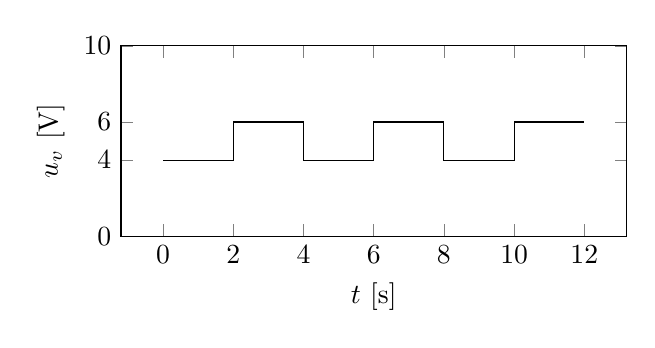
\begin{tikzpicture}
  \begin{axis}[
    width = 8cm,
    height = 4cm,
    ytick = {0,4,6, 10},
    xtick = {0,2, 4, 6, 8, 10, 12},
    ymin = 0,
    ymax = 10,
    ylabel = {$u_v$ [V]},
    xlabel = {$t$ [s]},
    ]

    \addplot[no marks] coordinates {(0,4) (2,4) (2,6) (4,6) (4, 4) (6, 4) (6,6) (8,6) (8,4) (10,4) (10,6) (12,6)};
    
  \end{axis}
\end{tikzpicture}
\end{document}
